\usetikzlibrary{arrows.meta}
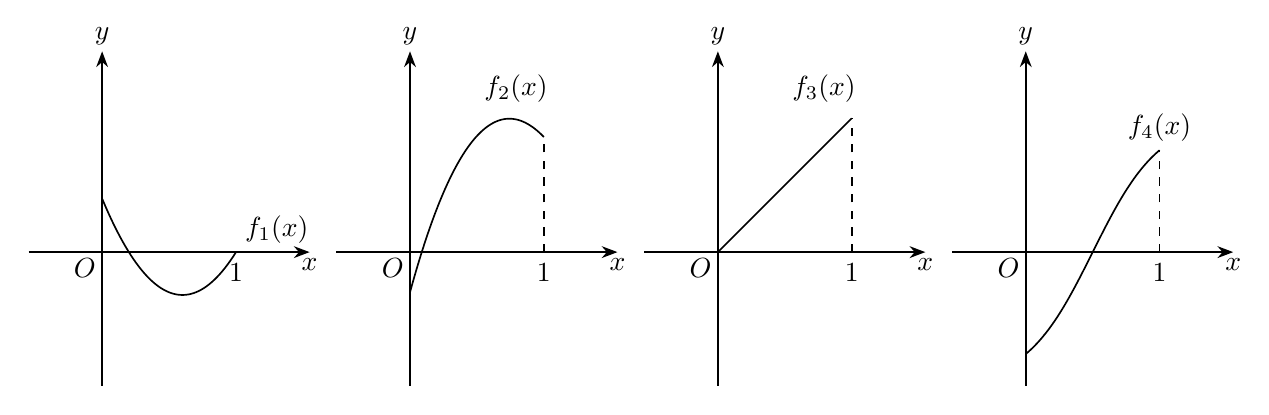
\begin{tikzpicture}[x=1.7cm,y=1.7cm,line width=.6pt,>=Stealth,font=\normalsize]
  \draw[->] (-0.55,0)--(1.55,0);
  \draw[->] (0,-1.0)--(0,1.5);
  \draw[->] (1.75,0)--(3.85,0);
  \draw[->] (2.3,-1.0)--(2.3,1.5);
  \draw[->] (4.05,0)--(6.15,0);
  \draw[->] (4.6,-1.0)--(4.6,1.5);
  \draw[->] (6.35,0)--(8.45,0);
  \draw[->] (6.9,-1.0)--(6.9,1.5);
  \node[anchor=north,inner sep=0pt,yshift=-2pt] at (1.55,0) {$x$};
  \node[anchor=north,inner sep=0pt,yshift=-2pt] at (3.85,0) {$x$};
  \node[anchor=north,inner sep=0pt,yshift=-2pt] at (6.15,0) {$x$};
  \node[anchor=north,inner sep=0pt,yshift=-2pt] at (8.45,0) {$x$};
  \node[anchor=south,inner sep=0pt,yshift=2pt] at (0,1.5) {$y$};
  \node[anchor=south,inner sep=0pt,yshift=2pt] at (2.3,1.5) {$y$};
  \node[anchor=south,inner sep=0pt,yshift=2pt] at (4.6,1.5) {$y$};
  \node[anchor=south,inner sep=0pt,yshift=2pt] at (6.9,1.5) {$y$};
  \node[anchor=north east,inner sep=0pt,xshift=-2pt,yshift=-2pt] at (0,0) {$O$};
  \node[anchor=north east,inner sep=0pt,xshift=-2pt,yshift=-2pt] at (2.3,0) {$O$};
  \node[anchor=north east,inner sep=0pt,xshift=-2pt,yshift=-2pt] at (4.6,0) {$O$};
  \node[anchor=north east,inner sep=0pt,xshift=-2pt,yshift=-2pt] at (6.9,0) {$O$};
  \node[anchor=north,inner sep=0pt,yshift=-4pt] at (1,0) {$1$};
  \node[anchor=north,inner sep=0pt,yshift=-4pt] at (3.3,0) {$1$};
  \node[anchor=north,inner sep=0pt,yshift=-4pt] at (5.6,0) {$1$};
  \node[anchor=north,inner sep=0pt,yshift=-4pt] at (7.9,0) {$1$};
  \node[anchor=south west,inner sep=0pt,xshift=3pt,yshift=3pt] at (1,0) {$f_1(x)$};
  \node[anchor=west,inner sep=0pt] at (2.85,1.22) {$f_2(x)$};
  \node[anchor=west,inner sep=0pt] at (5.15,1.22) {$f_3(x)$};
  \node[anchor=south,inner sep=0pt,yshift=3pt] at (7.9,.7616) {$f_4(x)$};
  \draw[domain=0:1,samples=121] plot (\x,{2*(\x-0.6)^2-0.32});
  \draw[dashed] (3.3,0)--(3.3,0.86);
  \draw[domain=2.3:3.3,samples=121] plot (\x,{0.3*(\x-2.3)^3-2.8*(\x-2.3)^2+3.66*(\x-2.3)-0.3});
  \draw[dashed] (5.6,0)--(5.6,1.0);
  \draw[domain=4.6:5.6,samples=2] plot (\x,{\x-4.6});
  \draw[dashed] (7.9,0)--(7.9,0.7616);
  \draw[domain=6.9:7.9,samples=241] plot (\x,{-1+2/(1+exp(-4*((\x-6.9)-0.5)))});
\end{tikzpicture}
